
\chapter{Referenzen zur Datenquelle 1}
    
    \section{Darstellung der Gesetzgebungsprozesse der EU}
    
    \begin{figure}[H]
        \centering
        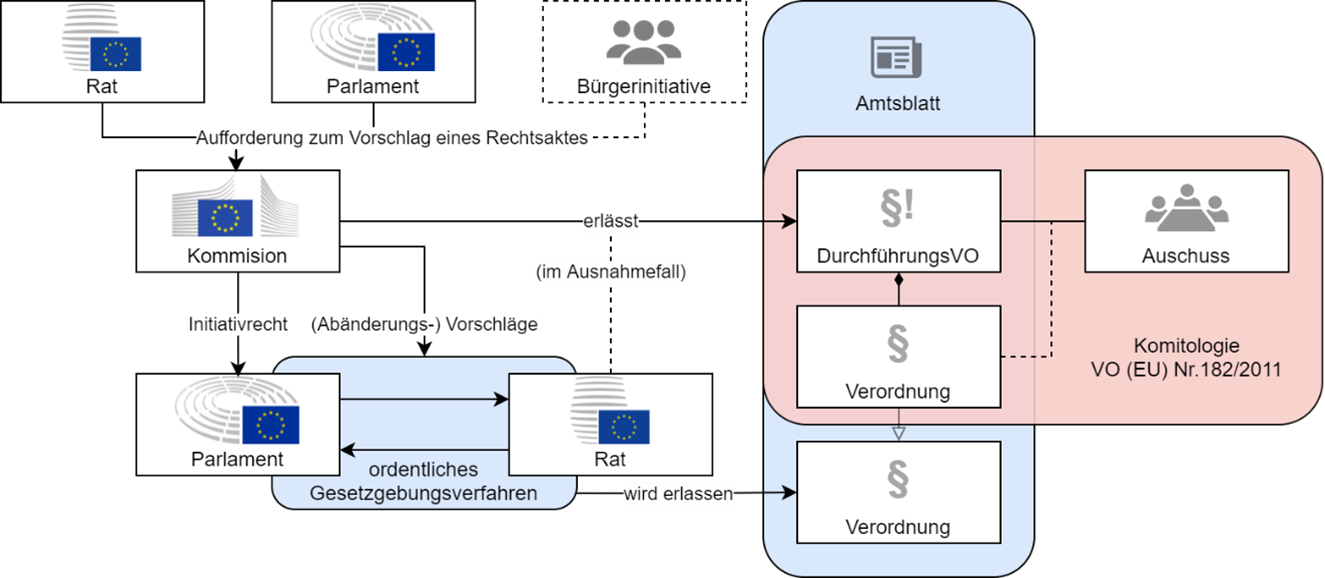
\includegraphics[width=\linewidth]{gfx/Gesegebungsprozess.png}
        \caption{Gesetzgebungsprozess der EU} 
        [Eigene Darstellung]
        \label{fig:europeg}
    \end{figure}

\section{Semantic Web Tech-Stack}
    
    \begin{figure}[H]
        \centering
        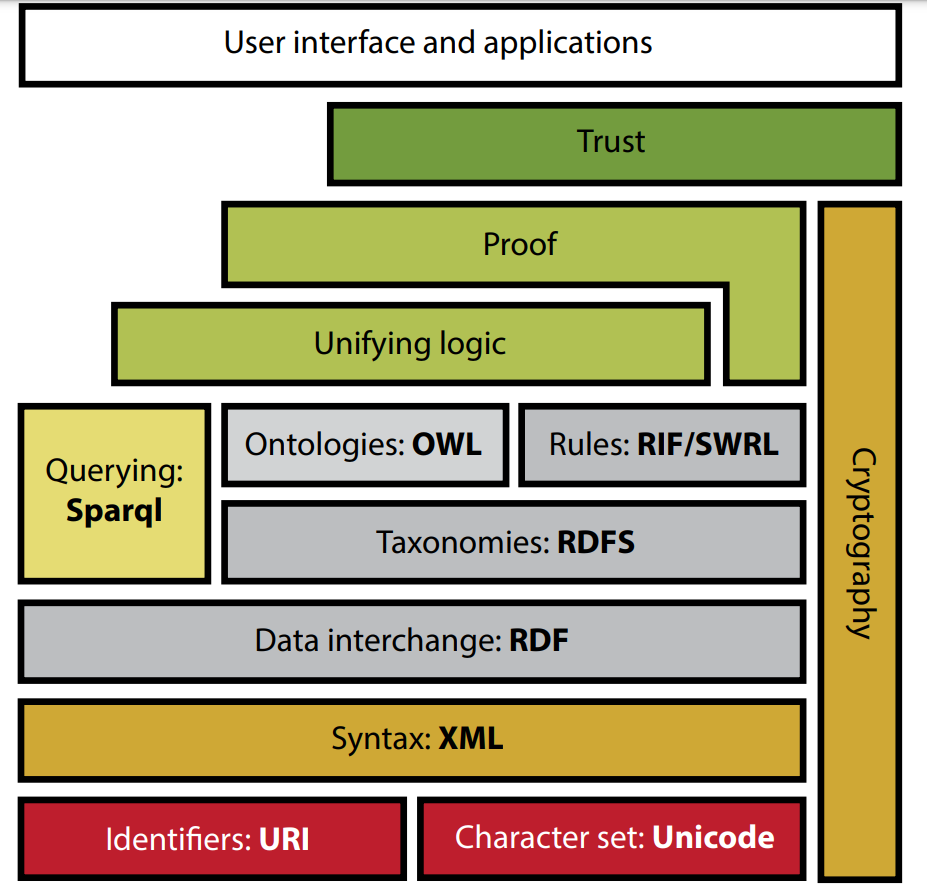
\includegraphics[width=.75\linewidth]{gfx/semantic_web_cake.png}
        \caption{Semantic Web Tech-Stack}\cite[10]{eu_cellar}\footnote{Ursprüngliche Quelle nach 2014 nicht mehr verfügbar}
        \label{fig:semantic}
    \end{figure}


\begin{lstlisting}[language=XML]
    <ANNOTATION>
        <TYPE_OF_LINK_TARGET>MS</TYPE_OF_LINK_TARGET>
        <ROLE2>{R|http://publications.europa.eu/resource/authority/fd_375/R}<ROLE2>
        <START_OF_VALIDITY>2020-11-05</START_OF_VALIDITY>
        <REFERENCE_TO_MODIFIED_LOCATION>
            {AN|http://publications.europa.eu/resource/authority/fd_370/AN} V
            {PO|http://publications.europa.eu/resource/authority/fd_370/PO} MET
            {PTA|http://publications.europa.eu/resource/authority/fd_370/PTA} (c) PT 1
        </REFERENCE_TO_MODIFIED_LOCATION>
    </ANNOTATION>
\end{lstlisting}


    % \begin{figure}
    %     \centering
    %     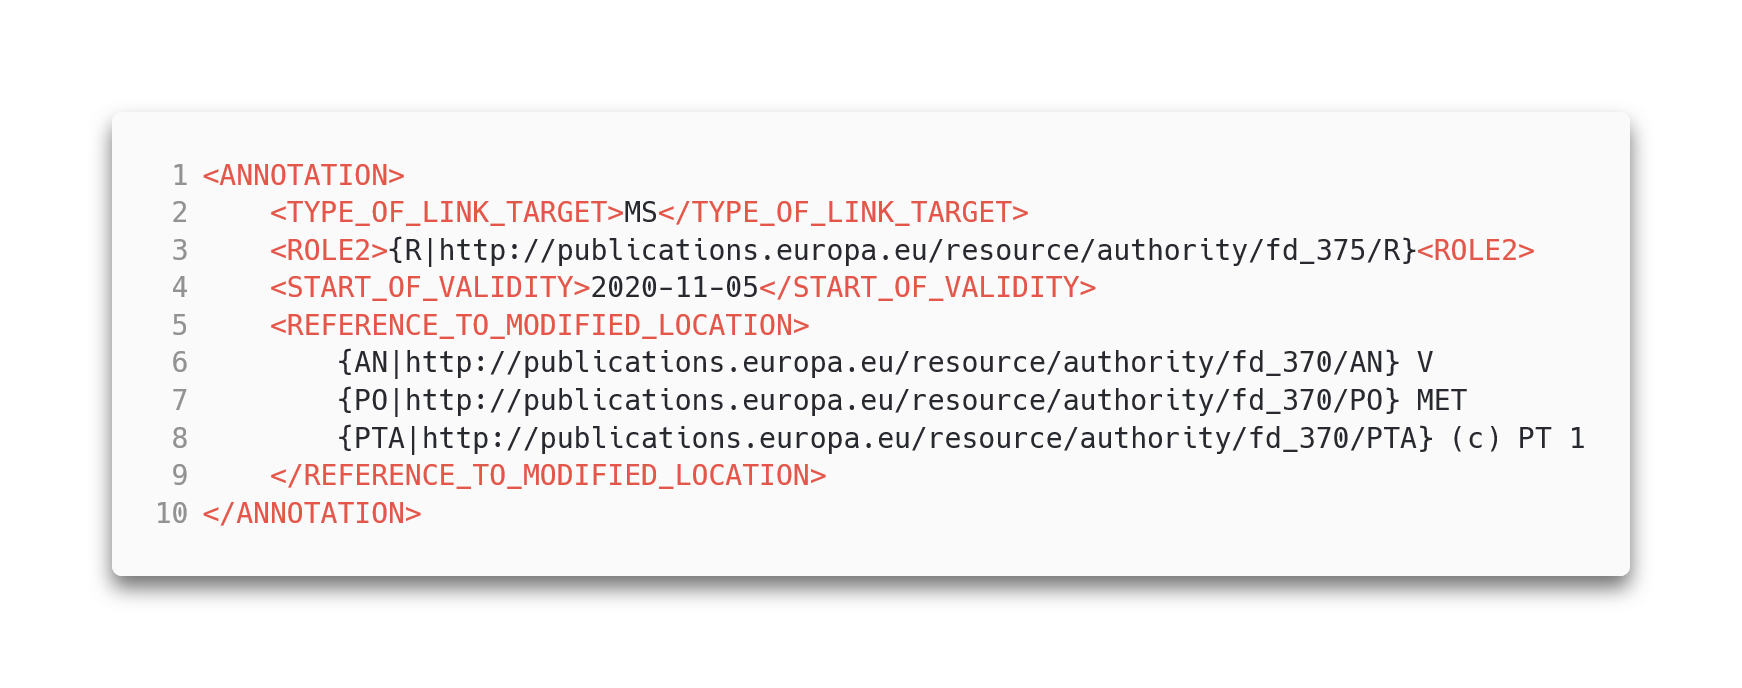
\includegraphics[width=\linewidth]{gfx/anno(1).png}
    %     \caption{}
    %     \label{fig:enter-label}
    % \end{figure}

    \pagebreak
    \section{Übersetzungen der referenzierten ATTO Tabellen}
    
    \begin{table}[H]
        \centering
        \begin{tabular}{|c|l|}\hline
            FD370 Code & Deutsche Übersetzung \\\hline \hline
            ADOPTION & Annahme \\\hline
            ALN & nicht nummerierter Absatz \\\hline
            AN & Anhang \\\hline
            APP & Anlage \\\hline
            AR & Artikel \\\hline
            C & C \\\hline
            CDR & AdR \\\hline
            CES & WSA \\\hline
            CHA & Kapitel \\\hline
            COL & Tabellenspalte \\\hline
            COMM & Kommission \\\hline
            CONS & Rat \\\hline
            CONSID & Erwägungsgrund \\\hline
            DU & vom \\\hline
            FR & Satz \\\hline
            JO & ABl. \\\hline
            L & L \\\hline
            OP\_DATPRO & Vorläufige Daten \\\hline
            P & S. \\\hline
            PA & Absatz \\\hline
            PBL & Präambel \\\hline
            PO & Nummer \\\hline
            PROT & Protokoll \\\hline
            PRT & Teil \\\hline
            PTA & Buchstabe \\\hline
            PTI & Ziffer \\\hline
            SBS & Unterabschnitt \\\hline
            SCT & Abschnitt \\\hline
            TAB & Tabelle \\\hline
            TIRE & Gedankenstrich \\\hline
            TIS & Titel (Gliederungsteil) \\\hline
            TIT & Titel \\\hline
            TXT & Text \\\hline
        \end{tabular}
        \caption{Deutsche Übersetzungen der Bezeichner der ATTO Tabelle FD\_370}
        \label{tab:fd_370}
    \end{table}
    
    \begin{table}[h]
        \centering
        \begin{tabular}{|c|l|}\hline
            FD375 Code & Deutsche Übersetzung \\\hline \hline
            A & Aufhebung \\\hline
            ADAP & Anpassung \\\hline
            % AF & Schlussakte \\\hline
            ANN & Anhang \\\hline
            AP & Teilweise Aufhebung \\\hline
            APA & Auch veröffentlicht als \\\hline
            % APP & Anlage \\\hline
            % APRO & Vorläufige Anwendung \\\hline
            % APRO/PART & Vorläufige teilweise Anwendung \\\hline
            % BJ & Rechtsgrundlage \\\hline
            C & Vervollständigung \\\hline
            CA & Hinfällig \\\hline
            % CH & Kapitel \\\hline
            CJ & Infragestellung der Rechtsgrundlage \\\hline
            CL\_VERSION & Konsolidierter Text \\\hline
            % CONF & Zustimmung \\\hline
            % CONSIDERANT & Erwägungsgrund \\\hline
            CPRJ & Ablehnung des gemeinsamen Standpunkts bestätigt \\\hline
            CREP & Erneute Anhörung \\\hline
            D & Abweichung \\\hline
            % DATE & Datum \\\hline
            % DATEFF & Datum des Inkrafttretens \\\hline
            DEL & Streichung \\\hline
            % DP & ab \\\hline
            DPR & Teilweise Ausnahme \\\hline
            E & Anwendung erweitert \\\hline
            % ECHLET & Briefwechsel \\\hline
            % EM & Mitgliedstaaten \\\hline
            % ET & und \\\hline
            % FIN & Finnland \\\hline
            I & Auslegung \\\hline
            % IRL & Irland \\\hline
            % IT & Italien \\\hline
            J & Zusatz \\\hline
            % JQ & bis \\\hline
            % L & Verbunden mit \\\hline
            M & Änderung \\\hline
            MD & Änderungsvorschlag \\\hline
            MNE & Nationale Durchführungsbestimmungen \\\hline
            MNV & Änderung für nichtig erklärt durch \\\hline
            NM & Ohne Änderungsvorschlag \\\hline
            O & Durchführung \\\hline
            OP\_DATPRO & Vorläufige Daten \\\hline
            P & Verlängerung \\\hline
            P/PART & Teilweise Fristverlängerung \\\hline
            % PA & Teil \\\hline
            PCRA & Billigung des gemeinsamen Entwurfs \\\hline
            PCRJ & Ablehnung des gemeinsamen Entwurfs \\\hline
            PI & Stillschweigende Verlängerung \\\hline
            PMD & Änderung des gemeinsamen Standpunkts \\\hline
            % PNM & Keine Änderung des gemeinsamen Standpunkts \\\hline
            % PRJ & Ablehnung des gemeinsamen Standpunkts \\\hline
            PROT & Protokoll \\\hline
            PROT.ADD & Zusatzprotokoll \\\hline
            % PSP & Teil des gleichen Verfahrens \\\hline
            % QUE/HOM & Entsprechende Anfrage \\\hline
            % QUE/PRE & Vorhergehende Anfrage \\\hline
            R & Ersetzung \\\hline
            R/PART & Teilweise Ersetzung \\\hline
            REP/COM & Ergänzende Antwort \\\hline
            REP/RECTIF & Berichtigende Antwort \\\hline
            % RJ & Ablehnende Stellungnahme \\\hline
            % RNV/HOM & Entsprechende Verweisung \\\hline
            % RNV/PAR & Teilweise Verweisung \\\hline
            RP & Wiedereinsetzung \\\hline
            S & Aussetzung \\\hline
            % SAUF & außer \\\hline
            SP & Teilweise Aussetzung \\\hline
            SU & Streichung \\\hline
            % T & Verspätete Anwendung \\\hline
            % TABL & Tabelle \\\hline
            % UK & Vereinigtes Königreich \\\hline
            % VERS.D & Deutscher Text \\\hline
            % VERS.DK & Dänischer Text \\\hline
            % VERS.EN & Englischer Text \\\hline
            % VERS.ES & Spanischer Text \\\hline
            % VERS.F & Französischer Text \\\hline
            % VERS.FI & Finnischer Text \\\hline
            % VERS.GR & Griechischer Text \\\hline
            % VERS.I & Italienischer Text \\\hline
            % VERS.NEM & Englischer / dänischer Text \\\hline
            % VERS.NL & Niederländischer Text \\\hline
            % VERS.PT & Portugiesischer Text \\\hline
            % VERS.S & Schwedischer Text \\\hline
            % VISA & Bezugsvermerke \\\hline
            % X & Wiedereinsetzung \\\hline
        \end{tabular}
        \caption{Deutsche Übersetzungen der Bezeichner der ATTO Tabelle FD\_375}
        (gekürzte Version)
        \label{tab:fd_375}
    \end{table}